% MAINTENANCE REVIEW/ACCEPTANCE
\chapter{4 MAINTENANCE REVIEW/ACCEPTANCE}

% 4.a OUTPUTS
\section{a. Sa�das}


% 1 New Baseline
\subsection{1 Nova baseline}
O novo sistema, bem como o kanban usado para o desenvolvimento das modifica��es encontram-se em reposit�rios no Github:

https://github.com/JosielFaleiros/gulosoo-back-end
https://github.com/JosielFaleiros/gulosoo-front-end

Sendo que na aba de "projects" � poss�vel ver o quadro do Kanban utilizado, como pode ser visto na imagem:

\begin{figure}
	\centering
	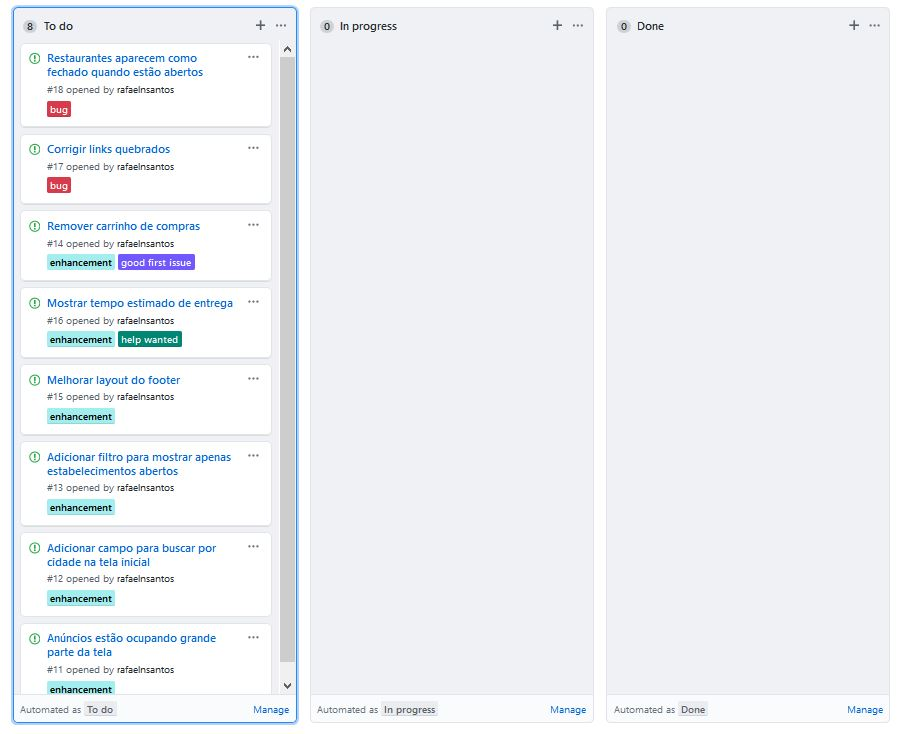
\includegraphics[width=0.7\linewidth]{images/kanban}
	\caption{Quadro Kanban da implementa��o das modifica��es}
	\label{fig:reporbgtest}
\end{figure}

\begin{figure}
	\centering
	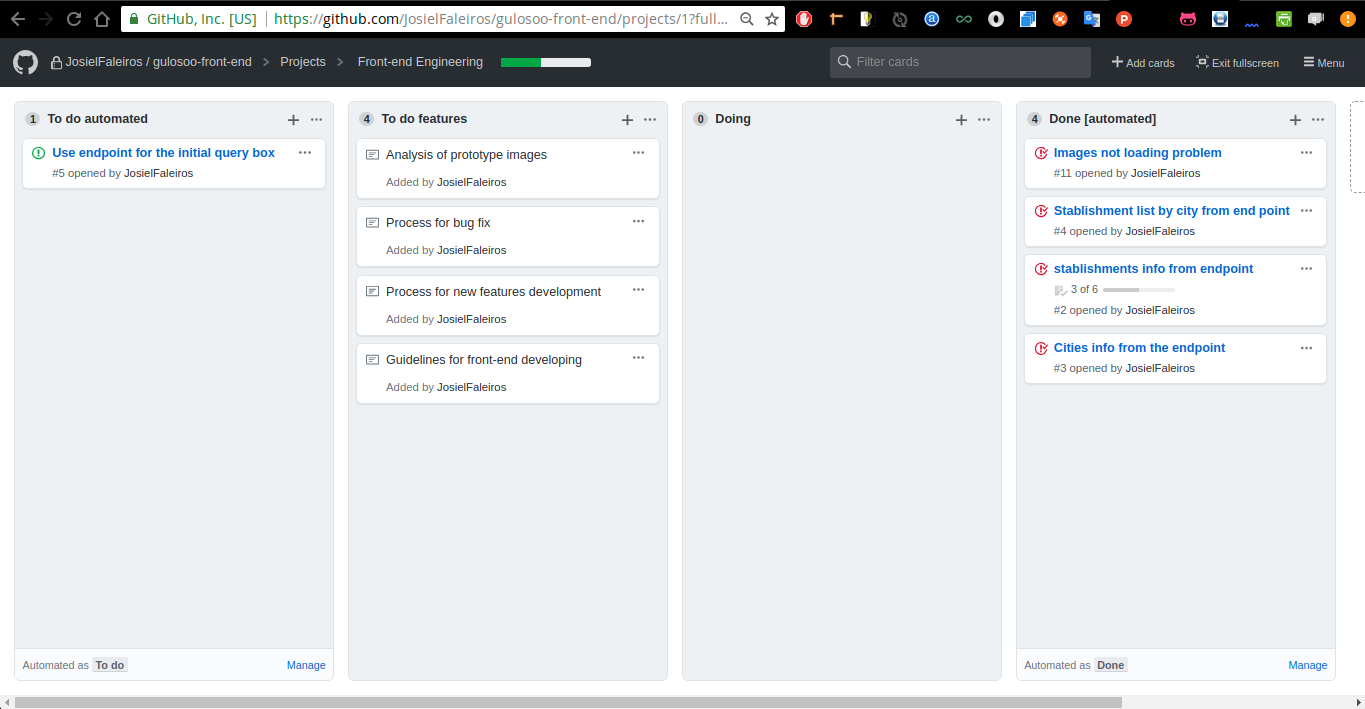
\includegraphics[width=0.7\linewidth]{images/front-end-project}
	\caption{Quadro Kanban da implementa��o da migra��o para o Vue JS}
	\label{fig:reporbgtest}
\end{figure}

\pagebreak


% 2 Rejected modfications
\subsection{2 Modifica��es rejeitadas}
Nenhuma modifica��o foi rejeitada.

% 3 An Acceptance report
\section{3 Um relat�rio de aceita��o}
Os testes automatizados geram os relat�rios que apresentam o sistema funcionando da forma esperada.


% 4 Audit and Review Reports
\section{4 Relat�rios de auditoria e aceita��o}
Como o sistema de versionamento GIT foi utilizado, � poss�vel rastrear cada altera��o realizada no sistema, possibilitando que o c�digo de uma modifica��o seje revertido para o estado anterior caso n�o seje aprovada.
Os testes automatizados geram os relat�rios que podem ser usados para analisar se o sistema se encontra em um estado de funcionamento esperado.

% 5 A Software Qualification Test Report
\section{5 Um relat�rio de teste de qualifica��o}
No projeto que est� no github possui  um README uma etiqueta indicando se os testes foram atendidos, onde o Travis executa automaticamente os testes e informa nesta etiqueta do README do github o estado dos testes, se passou ou n�o.